%$Header: /cvsroot/esrg/sfesrg/esrgpcpj/hyreach/doc/hyreachm/s_mfs0/s_mfs0.tex,v 1.6 2002/01/29 17:04:00 dtashley Exp $
%
%%%%%%%%%%%%%%%%%%%%%%%%%%%%%%%%%%%%%%%%%%%%%%%%%%%%%%%%%%%%%%%%%%%%%%%%%%%%%%%
%%%%%%%%%%%%%%%%%%%%%%%%%%%%%%%%%%%%%%%%%%%%%%%%%%%%%%%%%%%%%%%%%%%%%%%%%%%%%%%
%%%%%%%%%%%%%%%%%%%%%%%%%%%%%%%%%%%%%%%%%%%%%%%%%%%%%%%%%%%%%%%%%%%%%%%%%%%%%%%
\section{Modeling Framework Supported}
%Section Tag: MFS0.
\label{smfs0}

The modeling framework of \swname{} has been optimized for the 
computational efficiency of checking reachability properties
of a timing model of the interrupt subsystem of a software load.
This has two consequences:

\begin{itemize}
\item The modeling framework is severely constrained; i.e. all unnecessary
      expressiveness has been removed from the framework.
\item The modeling framework contains novel features (such as 
      the explicit definition of configuration equivalence classes) which are
	  not strictly necessary but which are a modeling convenience for the
	  particular category of problem that \swname{} was designed to address.
\end{itemize}

The modeling framework used is very close to that presented in 
\cite{bib:p:theoryofta:alurdill90}, with restrictions.  In this section,
we describe the modeling framework and the restrictions.


%%%%%%%%%%%%%%%%%%%%%%%%%%%%%%%%%%%%%%%%%%%%%%%%%%%%%%%%%%%%%%%%%%%%%%%%%%%%%%%
%%%%%%%%%%%%%%%%%%%%%%%%%%%%%%%%%%%%%%%%%%%%%%%%%%%%%%%%%%%%%%%%%%%%%%%%%%%%%%%
%%%%%%%%%%%%%%%%%%%%%%%%%%%%%%%%%%%%%%%%%%%%%%%%%%%%%%%%%%%%%%%%%%%%%%%%%%%%%%%
\subsection{Nomenclature}
%Subsection Tag: NMC0.
\label{smfs0:snmc0}

We adopt a nomenclature closer to that used
in \cite{bib:p:hybridsysintlat:lin90} than in \cite{bib:p:theoryofta:alurdill90}.
In most cases, terms are explained in more detail in Section \ref{sglo0}.

Generally, we seek to model the components which affect interrupt latency 
compatibility (software components such as critical sections and interrupt
service routines; as well as hardware components such as interrupt priority
resolution logic and communication peripherals) in a hybrid system framework.
In describing a system as \emph{hybrid}, we mean that its state vector is a mixture
of both discrete state and continuous state.

However, the systems we wish to evaluate for the absence or presence of certain
properties can be described without the full expressiveness
inherent in the notion of a hybrid system.  For example, in the software systems
of interest to us, the only continuous quantity of interest is usually time, and
thus all continuous variables in the system evolve at rate $\dot{x}_n = 1$ and it
isn't necessary to consider general differential equations.  The simplified framework
in which we model practical systems is the \emph{timed automata} framework as described
in \cite{bib:p:theoryofta:alurdill90}.


%%%%%%%%%%%%%%%%%%%%%%%%%%%%%%%%%%%%%%%%%%%%%%%%%%%%%%%%%%%%%%%%%%%%%%%%%%%%%%%
%%%%%%%%%%%%%%%%%%%%%%%%%%%%%%%%%%%%%%%%%%%%%%%%%%%%%%%%%%%%%%%%%%%%%%%%%%%%%%%
%%%%%%%%%%%%%%%%%%%%%%%%%%%%%%%%%%%%%%%%%%%%%%%%%%%%%%%%%%%%%%%%%%%%%%%%%%%%%%%
\subsection{Collection Of Cooperating EHMs}
%Subsection Tag: CCE0.
\label{smfs0:scce0}

The modeling framework accepted by \swname{} involves specifying a collection
of cooperating EHMs, $\{ \lambda_1, \ldots{}, \lambda_N \}$.  Each EHM $\lambda_i$
has 
two components to its state:

\begin{itemize}
\item A discrete component, which we call the \emph{configuration}.
\item Zero or more \emph{clocks}, $C_{ij}$, which can only assume
      non-negative integer values (Section \ref{smfs0:srit0}).
\end{itemize}

It is possible through a well-defined composition operation to combine all
EHMs into a CHM, which we denote $\Lambda$.  The CHM has the same design rules
as an EHM, but embodies the state space of all EHMs acting concurrently.

%%%%%%%%%%%%%%%%%%%%%%%%%%%%%%%%%%%%%%%%%%%%%%%%%%%%%%%%%%%%%%%%%%%%%%%%%%%%%%%
%%%%%%%%%%%%%%%%%%%%%%%%%%%%%%%%%%%%%%%%%%%%%%%%%%%%%%%%%%%%%%%%%%%%%%%%%%%%%%%
%%%%%%%%%%%%%%%%%%%%%%%%%%%%%%%%%%%%%%%%%%%%%%%%%%%%%%%%%%%%%%%%%%%%%%%%%%%%%%%
\subsection{Initial Conditions}
%Subsection Tag: ICO0.
\label{smfs0:sico0}

For modeling, each $\lambda_i$ has a unique initial configuration, which in figures we 
denote with a wedge (Fig. \ref{fig:smfs0:sico0:00}).  It is also assumed that 
every clock owned by every EHM starts with the value of 0.

\begin{figure}
\centering
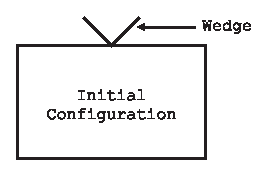
\includegraphics[height=1.0in]{s_mfs0/figini01.eps}
\caption{Initial Configuration Of EHM Depicted Using Wedge}
\label{fig:smfs0:sico0:00}
\end{figure}

For most practical models, the initial conditions described are adequate.
However, if different initial conditions are required, they can be 
created by 


%%%%%%%%%%%%%%%%%%%%%%%%%%%%%%%%%%%%%%%%%%%%%%%%%%%%%%%%%%%%%%%%%%%%%%%%%%%%%%%
%%%%%%%%%%%%%%%%%%%%%%%%%%%%%%%%%%%%%%%%%%%%%%%%%%%%%%%%%%%%%%%%%%%%%%%%%%%%%%%
%%%%%%%%%%%%%%%%%%%%%%%%%%%%%%%%%%%%%%%%%%%%%%%%%%%%%%%%%%%%%%%%%%%%%%%%%%%%%%%
\subsection{Restriction To Integer Time}
%Subsection Tag: RIT0.
\label{smfs0:srit0}


%%%%%%%%%%%%%%%%%%%%%%%%%%%%%%%%%%%%%%%%%%%%%%%%%%%%%%%%%%%%%%%%%%%%%%%%%%%%%%%
%%%%%%%%%%%%%%%%%%%%%%%%%%%%%%%%%%%%%%%%%%%%%%%%%%%%%%%%%%%%%%%%%%%%%%%%%%%%%%%
%%%%%%%%%%%%%%%%%%%%%%%%%%%%%%%%%%%%%%%%%%%%%%%%%%%%%%%%%%%%%%%%%%%%%%%%%%%%%%%
\subsection{Restriction To $\geq$ And $<$}
%Subsection Tag: RGE0.
\label{smfs0:srge0}


%%%%%%%%%%%%%%%%%%%%%%%%%%%%%%%%%%%%%%%%%%%%%%%%%%%%%%%%%%%%%%%%%%%%%%%%%%%%%%%
%%%%%%%%%%%%%%%%%%%%%%%%%%%%%%%%%%%%%%%%%%%%%%%%%%%%%%%%%%%%%%%%%%%%%%%%%%%%%%%
%%%%%%%%%%%%%%%%%%%%%%%%%%%%%%%%%%%%%%%%%%%%%%%%%%%%%%%%%%%%%%%%%%%%%%%%%%%%%%%
\subsection{Guards And Invariants}
%Subsection Tag: GAI0.
\label{smfs0:sgai0}


%%%%%%%%%%%%%%%%%%%%%%%%%%%%%%%%%%%%%%%%%%%%%%%%%%%%%%%%%%%%%%%%%%%%%%%%%%%%%%%
%%%%%%%%%%%%%%%%%%%%%%%%%%%%%%%%%%%%%%%%%%%%%%%%%%%%%%%%%%%%%%%%%%%%%%%%%%%%%%%
%%%%%%%%%%%%%%%%%%%%%%%%%%%%%%%%%%%%%%%%%%%%%%%%%%%%%%%%%%%%%%%%%%%%%%%%%%%%%%%
\subsection{Strong Synchronization (Events)}
%Subsection Tag: SSY0.
\label{smfs0:sssy0}


%%%%%%%%%%%%%%%%%%%%%%%%%%%%%%%%%%%%%%%%%%%%%%%%%%%%%%%%%%%%%%%%%%%%%%%%%%%%%%%
%%%%%%%%%%%%%%%%%%%%%%%%%%%%%%%%%%%%%%%%%%%%%%%%%%%%%%%%%%%%%%%%%%%%%%%%%%%%%%%
%%%%%%%%%%%%%%%%%%%%%%%%%%%%%%%%%%%%%%%%%%%%%%%%%%%%%%%%%%%%%%%%%%%%%%%%%%%%%%%
\subsection{Weak Synchronization (Guards Dependent On Configuration)}
%Subsection Tag: WSY0.
\label{smfs0:swsy0}


%%%%%%%%%%%%%%%%%%%%%%%%%%%%%%%%%%%%%%%%%%%%%%%%%%%%%%%%%%%%%%%%%%%%%%%%%%%%%%%
%%%%%%%%%%%%%%%%%%%%%%%%%%%%%%%%%%%%%%%%%%%%%%%%%%%%%%%%%%%%%%%%%%%%%%%%%%%%%%%
%%%%%%%%%%%%%%%%%%%%%%%%%%%%%%%%%%%%%%%%%%%%%%%%%%%%%%%%%%%%%%%%%%%%%%%%%%%%%%%
\subsection{Legal Versus Illegal Configurations}
%Subsection Tag: LVI0.
\label{smfs0:slvi0}


%%%%%%%%%%%%%%%%%%%%%%%%%%%%%%%%%%%%%%%%%%%%%%%%%%%%%%%%%%%%%%%%%%%%%%%%%%%%%%%
%%%%%%%%%%%%%%%%%%%%%%%%%%%%%%%%%%%%%%%%%%%%%%%%%%%%%%%%%%%%%%%%%%%%%%%%%%%%%%%
%%%%%%%%%%%%%%%%%%%%%%%%%%%%%%%%%%%%%%%%%%%%%%%%%%%%%%%%%%%%%%%%%%%%%%%%%%%%%%%
\subsection{Modeling Features Explicitly Not Supported}
%Subsection Tag: MEN0.
\label{smfs0:smen0}


%%%%%%%%%%%%%%%%%%%%%%%%%%%%%%%%%%%%%%%%%%%%%%%%%%%%%%%%%%%%%%%%%%%%%%%%%%
\noindent\begin{figure}[!b]
\noindent\rule[-0.25in]{\textwidth}{1pt}
\begin{tiny}
\begin{verbatim}
$RCSfile: s_mfs0.tex,v $
$Source: /cvsroot/esrg/sfesrg/esrgpcpj/hyreach/doc/hyreachm/s_mfs0/s_mfs0.tex,v $
$Revision: 1.6 $
$Author: dtashley $
$Date: 2002/01/29 17:04:00 $
\end{verbatim}
\end{tiny}
\noindent\rule[0.25in]{\textwidth}{1pt}
\end{figure}
%%%%%%%%%%%%%%%%%%%%%%%%%%%%%%%%%%%%%%%%%%%%%%%%%%%%%%%%%%%%%%%%%%%%%%%%%%
%$Log: s_mfs0.tex,v $
%Revision 1.6  2002/01/29 17:04:00  dtashley
%Version control info added, and minor edits.
%
%Revision 1.5  2001/10/31 04:31:37  dtashley
%Nightly safety checkin.
%
%Revision 1.4  2001/10/03 03:15:19  dtashley
%Nightly checkin.
%
%Revision 1.3  2001/10/02 03:16:54  dtashley
%Final edits evening of 10/01/01.
%
%Revision 1.2  2001/09/26 04:51:13  dtashley
%Edits.
%
%Revision 1.1  2001/09/26 02:31:14  dtashley
%Initial checkin, and some edits of main TEX file.
%
%End of S_MFS0.TEX.
